\documentclass[10pt]{article}
\usepackage{icmlko}

\icmlmeta{IP 파운데이션 월드모델}{297}{문턱을 넘었는데 조용하다}{팝업 학습을 16행에서 73행으로 늘려 청력 문턱을 처음 넘겼다 --- 이득은 여전히 0 이고 대신 출처 가드가 걸린다}

\begin{document}

\twocolumn[
\icmlheader

\begin{abstract}
노트 296이 팝업 학습 16행(F18 청력 22 아래)에서 ``이득이 아니라 흔들림''을
봤다. \textbf{문턱을 넘겨 봤다.} 팝업이 얇은 것은 자료가 없어서가 아니다 ---
\texttt{popup\_v2} 380행 중 2025 이전에 등급 A·B \textbf{그리고}
\texttt{scope\_usable} \textbf{그리고} 라벨 유한인데 \textbf{세는 법이
\texttt{organizer\_claim}} 이라 빠지는 행이 \textbf{53개}다. 풀면 학습
16$\to$\textbf{73}, 청력 22를 처음으로 넘는다. 그런데 재료를 읽어 보니
\textbf{그 판이 이미 있었다}(\texttt{lab/loop.py} 의 \texttt{\_wide},
노트 127 · 133). 노트 127은 분모를 59에 고정하고도 팝업이
$+$0.3688$\to+$0.4495 로 오른다고 적었다. \textbf{그래서 물음을 바꿨다} ---
오늘 만든 가드 19(출처)에 \texttt{wide\_trendcal} 과
\texttt{wide\_trendcalpop} 이 걸린다(노트 292). \textbf{노트 127의 이득이
표지였나?} 재기 전에 ``걸릴 것 같다''를 적고 쟀다. 챔피언 축 세트를 넓힌
\texttt{wide\_tcwt} 를 처음 만들어 재니 \textbf{가드 19가 걸린다} --- 팝업 축
8개가 검색·공유 두 계열을 가로질러 함께 결측하고 그 무늬가 라벨과
$\rho{=}{-}0.387$ 이다. 그리고 \textbf{분모를 59에 고정하면 이득이 거의
없다}: 좁힘 $+$0.3324 $\to$ 넓힘 $+$0.3440, 차 \textbf{$+$0.0116} 에 짝SE
\textbf{0.0849}, $t{=}{+}0.14$ --- \textbf{검출 문턱 0.17 의 열네 분의 일}이다.
\textbf{청력 문턱은 필요조건이었지 충분조건이 아니었다.} 그리고 이 분모
(유보 59행)에서는 \textbf{$+$0.08 짜리 이득도 0 과 못 가른다} --- 노트 127이
보고한 수가 정확히 그 크기다.
\end{abstract}
]

\section{팝업이 얇은 것은 자료가 없어서가 아니다}

노트 296이 남긴 갈래는 ``팝업 학습 행 늘리기 --- 16$\to$22 면 F18 이
듣는다''였다. 어디까지 늘릴 수 있는지 셌다.

\begin{center}\footnotesize
\begin{tabular}{lrr}
\hline
\texttt{popup\_v2} 380행 & 전체 & 2025 이전 \\
\hline
라벨 유한 & 350 & 148 \\
등급 A·B & 204 & 84 \\
\texttt{scope\_usable} & 353 & 158 \\
세는 법 \texttt{entry}/\texttt{participation} & 91 & \textbf{26} \\
\hline
넷 다 통과 & 75 & \textbf{16} \\
\hline
\end{tabular}
\end{center}

\textbf{병목은 세는 법 하나다.} 2025 이전에 등급 A·B 이고
\texttt{scope\_usable} 이고 라벨도 있는데 \textbf{세는 법이
\texttt{organizer\_claim}} 이라 빠지는 행이 \textbf{53개}다. 풀면 학습
16$\to$\textbf{73} 이고 F18 의 청력 22를 넘는다.

\textbf{그러니 팝업이 얇은 것은 라벨 기준을 지킨 결과다.}

\section{그런데 그 판이 이미 있었다}

\texttt{lab/loop.py} 에 \texttt{\_wide} 가 있다. 노트 127 · 133이 만든
것이고, 노트 127은 \textbf{분모를 원래 59건에 고정해 놓고도} 팝업이
$+$0.3688 $\to$ $+$0.4495 로 오른다고 적었다.

\textbf{그래서 물음을 바꿨다.} 오늘 노트 292가 만든 가드 19(출처)에
\texttt{wide\_trendcal} 과 \texttt{wide\_trendcalpop} 이 \textbf{걸린다.}
그 가드는 \emph{한 도메인에 자료원이 둘 섞였나}를 본다 ---
\texttt{organizer\_claim} 행과 \texttt{entry} 행은 손 축 마스크 무늬가 다르고,
무늬가 출처를 가리키고 출처가 라벨을 가르면 모형은 축이 아니라 출처를
배운다(노트 266의 덫, 노트 283이 시장 팝업을 따로 연 이유).

\textbf{노트 127은 가드 19가 없던 때의 측정이다.}

\paragraph{예측을 적고 쟀다} \texttt{preregister\_popuphear.json}:
``\textbf{걸릴 것이라고 본다} --- 축 세트를 wiki·tag 로 늘리는 것이 출처
무늬를 없애지는 않는다.'' 그리고 ``가드 19가 걸리면 이득이 얼마든 무효로
적는다.''

\section{걸렸다. 그리고 이득도 없다}

\begin{figure*}[t]
\centering
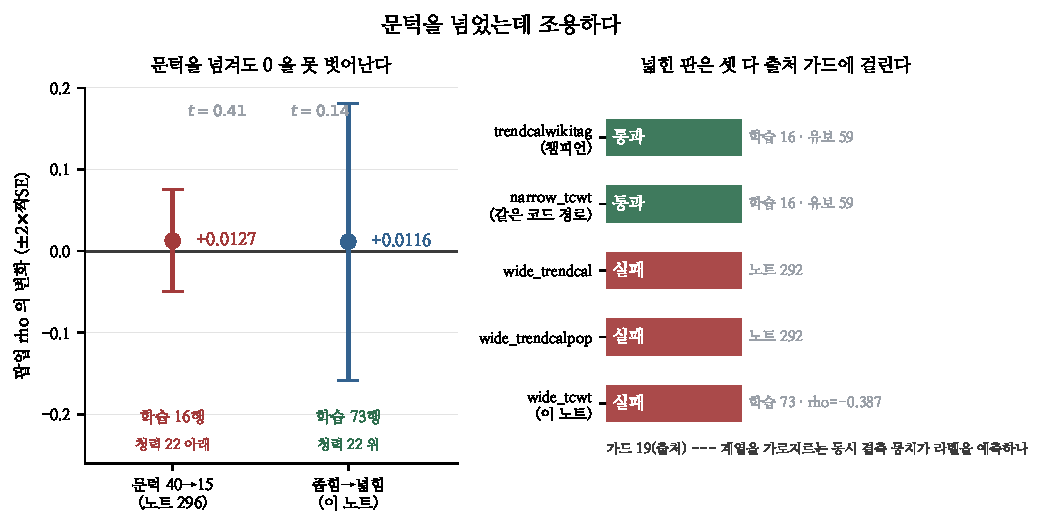
\includegraphics[width=\textwidth]{figs/crossed.pdf}
\caption{왼쪽 --- 청력 문턱 아래(노트 296)와 위(이 노트)에서 잰 팝업 $\rho$
변화. 오른쪽 --- 가드 19(출처) 판정.}
\end{figure*}

챔피언 축 세트를 넓힌 \texttt{wide\_tcwt} 를 처음 만들어 쟀다.

\begin{center}\footnotesize
\begin{tabular}{lrrl}
\hline
축 세트 & 학습 & 유보 & 가드 19 \\
\hline
\texttt{trendcalwikitag} & 16 & 59 & \textbf{통과} \\
\texttt{narrow\_tcwt} & 16 & 59 & \textbf{통과} \\
\texttt{wide\_tcwt} & 73 & 116 & \textbf{실패} \\
\hline
\end{tabular}
\end{center}

\begin{center}\footnotesize
가드 19: ``팝업 축 8개가 계열 \emph{검색}/\emph{공유} 를 가로질러 함께 결측,
$\rho{=}{-}0.387$''
\end{center}

\textbf{예측대로 걸렸다.} 여덟 축이 두 계열을 가로질러 같이 비고, 그 결측
무늬가 라벨을 $\rho{=}{-}0.387$ 로 가른다. 축이 아니라 \textbf{출처}를 가리키는
열이다.

\paragraph{그리고 분모를 고정하면 이득이 없다} 넓힌 판은 유보도 59$\to$116
으로 늘어난다 --- 그건 과제가 바뀐 것이라 그대로 견주면 안 된다(노트 284).
공통 유보 \textbf{59행}에서 다시 쟀다.

\begin{center}\small
\begin{tabular}{lr}
\hline
좁힘(\texttt{narrow\_tcwt}) & $+$0.3324 \\
넓힘(\texttt{wide\_tcwt}) & $+$0.3440 \\
\hline
차 & \textbf{$+$0.0116} \\
짝SE & \textbf{0.0849} \\
$t$ & $+$0.14 \\
검출 문턱 & \textbf{0.1697} \\
\hline
\end{tabular}
\end{center}

\textbf{문턱의 열네 분의 일이다.} 학습 행을 16에서 73으로 \emph{네 배 반}
늘리고 청력 문턱을 처음 넘겼는데 \textbf{아무 일도 안 일어났다.}

\section{그래서 두 가지가 정리된다}

\paragraph{① 청력은 필요조건이지 충분조건이 아니다} 노트 296은 문턱
\emph{아래}에서 ``이득 없음 · 큰 흔들림''을 봤다. 이 노트는 문턱 \emph{위}에서
``이득 없음''을 본다. \textbf{문턱을 넘는 것은 배울 수 있게 하는 것이지
배울 것이 있게 하는 것이 아니다.}

\paragraph{② 팝업에서 $+$0.08 은 애초에 못 재는 크기다} 좁힘$\to$넓힘을
유보 59행에서 재면 짝SE 가 \textbf{0.0849} --- 문턱 \textbf{0.1697} 이다.
노트 127이 보고한 $+$0.0807 은 \textbf{그 절반}이다.

\begin{center}\footnotesize
\begin{tabular}{lrr}
\hline
& 이득 & 문턱 \\
\hline
297 좁힘$\to$넓힘 (\texttt{tcwt}) & $+$0.0116 & \textbf{0.1697} \\
296 문턱 40$\to$15 (\texttt{tcwt}) & $+$0.0127 & 0.0624 \\
\hline
127 좁힘$\to$넓힘 (다른 축 세트) & $+$0.0807 & 안 쟀다 \\
\hline
\end{tabular}
\end{center}

\textbf{노트 127의 문턱을 그대로 안다고 말할 수는 없다} --- 축 세트가 달라
짝SE 를 다시 재야 한다. 다만 \emph{같은 분모(유보 59행) · 같은 대조(좁힘 대
넓힘)}이고 이쪽에서 0.17 이 나온다. \textbf{그러니 $+$0.0807 을 이득으로 읽으려면
그 판에서 짝SE 를 재서 보여야 한다.} 노트 127을 지우지 않는다 --- 그때의
측정이 틀렸다는 것이 아니라 \textbf{그 크기를 갈랐다고 말할 근거가 아직
제시된 적이 없다}는 것이다.

\paragraph{남은 것}
\begin{center}\small
\begin{tabular}{ll}
\hline
갈래 & 왜 \\
\hline
하네스 셋 넓히기 & +57건 끝남 --- 다음 노트 \\
팝업 유보를 늘릴까 & 문턱이 유보 59행에서 온다 \\
넓힌 판을 은퇴시킬까 & 가드 19 실패 · 이득 미검출 \\
lab 회사 축 & 노트 294의 $+$0.0040 \\
\hline
\end{tabular}
\end{center}

\paragraph{규약} \textbf{옛 노트의 이득을 지금 문턱으로 다시 재라.} 이
실험실이 넓힌 팝업 판을 갖게 된 근거가 노트 127의 $+$0.0807 인데, 같은
분모 · 같은 대조를 오늘 재면 문턱이 0.17 이다. 문턱을 재는 법(노트 274)이
그때는 없어서 짝SE 를 아무도 안 적었다. \textbf{도구가 생기면 도구가 없던 때의 결론을 다시 통과시켜야
한다} --- 오늘 가드 19가 \texttt{wide} 셋을 전부 걸러 낸 것도 같은 일이다.

\end{document}
